\chapter{Theory} \label{sec:theory}
\section{Ultrasound}

\begin{figure}[ht]
	\centering
	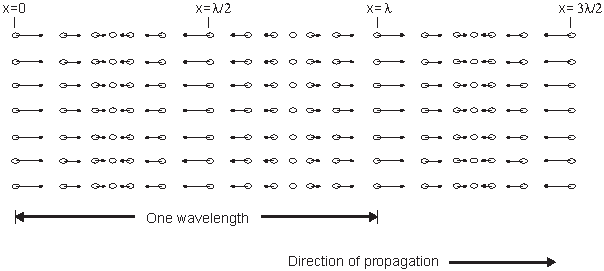
\includegraphics[width=\textwidth]{2_plane_wave_jensen-cropped.pdf}
	\caption[Particle displacement for a propagating ultrasound wave]{Particle displacement for a propagating ultrasound wave \cite{JensenUltrasoundBook}}
	\label{fig:2_planewave_jensen}
\end{figure}

\gls{us} is a technology that transmit sound wave with frequencies above the audible range (\qtyrange[range-units = single]{20}{20e3}{\hertz}) to mechanically vibrate matter. The particles in the medium would be at rest and distributed uniformly before any disturbance. The wave propagates as a disturbance and the particles oscillate around their mean position due to the presence of the ultrasonic wave. Typically the \gls{us} frequency band used in clinical settings are from \qtyrange[range-units = single]{1}{15}{\mega\hertz} \cite{Szabo_UltrasoundBook_2}. \Cref{fig:2_planewave_jensen} visualizes the propagation of a plane wave in matter. The oscillation occurs parallel to the wave's direction, making it longitudinal, and the disturbance will propagate with the variable $c$, which is determined by the medium and is given by \cref{eq:2_velocity_c}.
\begin{equation} \label{eq:2_velocity_c}
	c = \sqrt{\frac{1}{\rho_{0} \kappa_{S}}}
\end{equation}
Where $\rho_{0}$ is the mean density (\unit{\kilogram\per\meter\cubed}) and $\kappa_{S}$ is the \gls{adiabatic} compressibility (\unit{\meter\squared\per\newton}). Since in the majority of cases, the propagation of ultrasound is linear, it is assumed in this work. 

The acoustic pressure of the harmonic plane wave is expressed by \cref{eq:2_acoustic_pressure}
\begin{equation} \label{eq:2_acoustic_pressure}
	p(t,z)=p_{0} e^{j(\omega t - k z)}
\end{equation}
And propagates along the $z$-axis. $\omega$ is the angular frequency, $k$ is the wave number and is expressed by $k=\nicefrac{\omega}{c}=\nicefrac{2\pi}{\lambda}$, and $_{0}$ is the acoustic pressure amplitude. A spherical wave is expressed by \cref{eq:2_spherical_wave}
\begin{equation} \label{eq:2_spherical_wave}
	p(t,r)=p_{0} e^{j(\omega t - k r)}
\end{equation}
Where $r$ is radial distance, and is defined in a polar coordinate system. For each time instance, the acoustic pressure $p(t,r)$ is constant over a fixed radial position. In this scenario, the pressure amplitude is given by $p_{0}(r) = \nicefrac{k_{p}}{r}$, where $k_{p}$ is a constant since the energy of the outgoing wave must be constant.  Particle speed $u$ is dependent on the pressure caused by a wave expressed by \cref{eq:2_particle_speed}
\begin{equation} \label{eq:2_particle_speed}
	u = \frac{p}{Z}
\end{equation}
Where $Z$ is the characteristic acoustic impedance, defined as the ratio of acoustic pressure to particle speed at a given position in the medium and is expressed by \cref{eq:2_acoustic_impedance}.
\begin{equation} \label{eq:2_acoustic_impedance}
	Z = \rho_{0} c
\end{equation}

Characteristic acoustic impedance $Z$ is one of the most significant variables in the characterization of propagating plane waves. Reference values for density, speed of sound, and characteristic acoustic impedance can be seen in \cref{tab:2_density_tissue}.

\begin{table}[ht]
	\centering
	\caption[Approximate density, sound speed, and acoustic impedance of human tissue types]{Approximate density, sound speed, and acoustic impedance of human tissue types \cite{JensenUltrasoundBook}}
	\label{tab:2_density_tissue}
	\sisetup{range-phrase=--,range-exponents = combine}
	\begin{tblr}[]{ 
		colspec = {XSSS}, width = \linewidth,
		row{1} = {guard,m,font=\small\bfseries},
%			column{2,3,4} = {r},
		}
		\toprule
		Medium & {Density ($\rho_{0}$)\\\unit[per-mode = symbol]{\kilogram\per\meter\cubed}} & {Speed of sound ($c$)\\\unit[per-mode = symbol]{\meter\per\second}} & {Characteristic\\\textbf{acoustic impedance ($Z$)}\\\unit[per-mode = symbol]{\kilogram\per\meter\squared\per\second}} \\ \midrule
		Air             & 1.2     & 333            & 0.4e3       \\
		Blood           & 1.06e3    &    1566        &  1.66e6     \\
		Bone            & \numrange{1.38e3}{1.81e3}  &   \numrange{2070}{5350}{}       & \numrange{3.75e6}{7.38e6}{} \\
		Brain           &  1.03e3       & \numrange{1505}{1612}{}  & \numrange{1.55e6}{1.66e6}{} \\
		Fat             &  0.92e3  &  1446 & 1.33e6 \\
		Kidney          &  1.04e3  & 1567 & 1.62e6 \\
		Lung            &  0.4e3  &  650  & 0.26e6 \\
		Liver           &  1.06e3  &  1566  & 1.66e6 \\
		Muscle          &  1.07e3  & \numrange{1542}{1626}{} & \numrange{1.65e6}{1.74e6}{} \\
		Spleen          &  1.06e3  & 1566 & 1.66e6 \\
		Distilled water &  1e3  & 1480 & 1.48e6 \\ \bottomrule
	\end{tblr}
\end{table}

In the following sections, various acoustic wave phenomena will be briefly described.

\subsection{Scattering}
A wave propagating across a medium continues in the same direction until it encounters a new medium. When this occurs, a portion of the wave is transmitted into the new medium, with a change in direction. Because the scattered wave is the result of several contributors, it is necessary to define it statistically. The amplitude distribution is Gaussian \cite{JensenUltrasoundBook} and can thus be fully described by its mean and variance. The mean value is zero because the dispersed signal is caused by variances of the acoustic characteristics in tissue.

The correlation between multiple data is what allows ultrasound to determine blood velocities.
Because minor movements have a significant correlation, it is feasible to discover alterations in location by comparing sequential measurements of moving structure, such as blood cells. In medical ultrasound, just one transducer is utilised for transmitting and receiving, and only the backscattered signal is analysed. 

The power of scattered signal is defined by the scattering cross-section, which in small cases mean a uniform intensity $I_{i}$, and is expressed by \cref{eq:2_scatter_power}.
\begin{equation} \label{eq:2_scatter_power}
	P_{s} = I_{i} \sigma_{s c}
\end{equation}
Where $\sigma_{s c}$ is the scattering cross-section in square meters. The backscattering cross section is material dependant and determines the intensity of the scattering. If the dispersed energy is evenly emitted in all directions, the scattered intensity is given by \cref {eq:2_scatter_intensity}.
\begin{equation} \label{eq:2_scatter_intensity}
	I_{s} = \frac{P_{s}}{4 \pi R^{2}} = \frac{\sigma_{sc}}{4 \pi R^{2}} \cdot I_{i}
\end{equation}
Where $R$ is distance to the scattering region \cite{JensenUltrasoundBook}. This results in a spherical wave. A transducer with radius $r$ gives the power $P_{r}$, presuming the attenuation and focus is neglected, and is expressed by \cref{eq:2_transducer_r_power}.
\begin{equation} \label{eq:2_transducer_r_power}
	P_{r} = I_{s} \pi r^{2} = \sigma_{s c} \frac{r^{2}}{4 R^{2}} \cdot I_{i}
\end{equation}

The backscattering coefficient, which characterizes scattering from a volume of scatterers, is another measure of scattering strength. It is defined as average received power per steradian volume of scatterers when flooded with plane waves of unit amplitude and the unit is \unit{1\per\centi\meter\steradian}.

Back scattering coefficients in blood are significantly lower than the back scattering coefficients from various tissue types. This poses a challenge when estimating blood flow close to tissue vessel walls \cite{ShungScattering1992,JensenUltrasoundBook}.

\subsection{Attenuation}
The ultrasonic wave will be reduced as it propagates through tissue due to absorption and scattering. The attenuation in tissue is frequency dependent, with greater attenuation with increasing frequency. Because of absorption and dispersion, the ultrasonic wave will be attenuated as it travels through tissue. The relationship between attenuation, distance traveled, and frequency is frequently linear. Attenuation in tissue occurs as a result of both dispersion, which spreads energy in all directions, and absorption, which turns it to thermal energy. 

\begin{table}[ht]
	\centering
	\caption[Approximate attenuation values for human tissue]{Approximate attenuation values for human tissue
		\cite{JensenUltrasoundBook}}
	\label{tab:my_label}
	\sisetup{range-phrase=--,range-exponents = combine}
	\begin{tblr}[]{%
			width=.3\textwidth,
			colspec = {
				*{1}{X[2]}
				*{1}{S[]}
			},
			row{1} = {guard, m, font=\small\bfseries},
			measure=vbox, stretch=-1,
			%vlines, hlines,
		}
		\toprule
		Tissue & {Attenuation \\ $\unit[per-mode = symbol,inter-unit-product =\cdot]{\dB\per\mega\hertz\per\centi\meter}$ } \\ 
		\midrule
		Liver & \numrange{0.6}{0.9}{} \\
		Kidney & \numrange{0.8}{1}{} \\
		Spleen & \numrange{0.5}{1}{}\\
		Fat & \numrange{1}{2}{} \\
		Blood & \numrange{0.17}{0.24}{} \\
		Plasma & 0.01 \\
		Bone & \numrange{16}{23}{} \\
		\bottomrule
	\end{tblr}
\end{table}

The pressure of a wave propagating in $z$-direction decreases exponentially expressed by \cref{eq:2_attenuation_pressure}
\begin{equation} \label{eq:2_attenuation_pressure}
	p(z) = p(z=0) e^{-\alpha z}
\end{equation}
Where $p(z=0)$ is the pressure in the point of origin and $\alpha$ is the attenuation coefficient. The attenuation coefficient unit is \si{\neper\per\centi\meter} and alternatively, \si{\dB\per\centi\meter} with the relationship described in \cref{eq:2_attenuation_coefficient}. 

\begin{subequations} \label{eq:2_attenuation_coefficient}
	\begin{align}
		\ensuremath{\alpha &= \frac{1}{z} \ln \frac{p(z=0)}{p(z)} \\
		\alpha( \si{\dB\per\centi\meter} ) &= 20 ( log_{10}e) \alpha ( \si{\neper\per\centi\meter}) = 8.68\alpha (\si{\neper\per\centi\meter})}
	\end{align}
\end{subequations}

The significance of absorption and scattering in ultrasonic attenuation in biological tissues is a point of contention. Scattering adds just a few percent to attenuation in most soft tissues. As a result, it is fair to conclude that absorption is the primary mechanism for ultrasonic attenuation in biological tissues \cite{ShungUltrasound_Book}.

\subsection{Transducer}

\begin{figure}[ht]
	\centering
	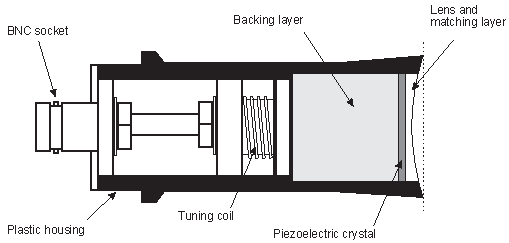
\includegraphics[width=.6\textwidth]{2_transducer_construction-cropped.pdf}
	\caption[Single element ultrasound transducer construction]{Single element ultrasound transducer construction \cite{JensenUltrasoundBook}}
	\label{fig:2_transducer_construction}
\end{figure}

A layperson knows transducers as speakers and microphones in the context of PA systems. In the case of medical \gls{us} it is the device that generates the acoustic pressure field, which is emitted into tissue. The transducer has a piezoelectric crystal inside the housing. When excited, this crystal emits ultrasound waves toward flowing blood. The red blood cells will reflect a fraction of the emitted waves. These reflected waves are of a different frequency than the transmitted wave. If the red blod cells are moving away from the transducer, the frequency will be lower. If the red blod cells are moving towards the transducer, the frequency will be higher. This is caused by the \gls{doppler}. The reflected ultrasonic waves return to the crystal and are converted back into electrical signals. The single element transducer shown in \cref{fig:2_transducer_construction} has a minimal imaging window and has to be mechanically manipulated to get a wide window, which is unfeasible for responsive high-frequency imaging. Thus, usually an array transducer is used. Various \gls{us} transducer types exist with different strengths and weaknesses, shown in \cref{fig:2_transducer_types}. 

\begin{figure}[ht]
	\centering
	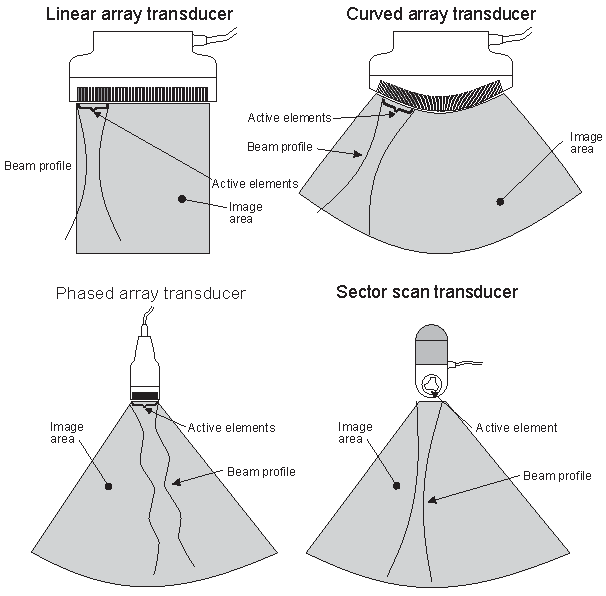
\includegraphics[width=.8\textwidth]{2_transducer_types-cropped.pdf}
	\caption[Transducer types for acquiring B-mode images]{Transducer types for acquiring B-mode images \cite{JensenUltrasoundBook}}
	\label{fig:2_transducer_types}
\end{figure}

\subsection{Doppler effect} \label{sec:doppler_effect}

\begin{figure}[ht]
	\centering
	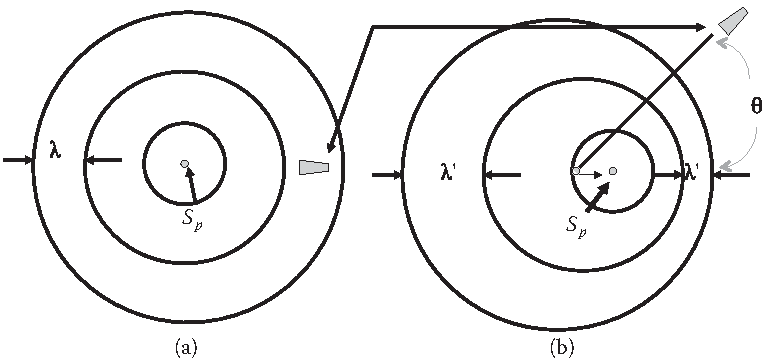
\includegraphics[width=.8\textwidth]{2_doppler_shung-cropped.pdf}
	\caption[Doppler effect diagram]{Doppler effect diagram. A stationary observer perceives a change in frequency of a wave generated by a moving source toward the observer as a result of a wavelength shift from $\lambda\ $ to $\lambda^{\prime}$. In (a), the source is still. In (b), the source is moving at a velocity $v$. \cite{ShungUltrasound_Book}}
	\label{fig:2_doppler_effect}
\end{figure}

The Doppler effect is a phenomena in which an observer perceives a shift in the frequency of sound emitted from a source when either the source or the observer is moving, or both are moving. The reason for the perceived change in frequency is visualised in \cref{fig:2_doppler_effect}. In diagram (a), the source $S_{p}$ is stationary and producing a spherical distribution pattern of the wave with the perceived frequency of the observer is given by $f=\nicefrac{c}{\lambda}$, where $c$ is the velocity of the wave in the medium and $\lambda$ is the wavelength. In diagram (b), the sound source is moving towards the right with a velocity $v$. The locomotion of the source changes the distribution pattern and causes a longer wavelength on the left, indicating a lower perceived frequency, and a shorter wavelength on the right, indicating a higher perceived frequency, both denoted as $\lambda^{\prime}$ in the diagram.

In the case of the observer on the right side, the perceived frequency becomes \cref{eq:2_doppler_effect}.

\begin{equation} \label{eq:2_doppler_effect}
	f^{\prime} = \frac{c}{\lambda} = \frac{c}{\lambda - v T} = \frac{c}{(c-v)T} = \frac{c}{c-v}\cdot f_{0}
\end{equation}
And viceversa, on the left side, the perceived frequency becomes \cref{eq:2_doppler_effect2}.
\begin{equation} \label{eq:2_doppler_effect2}
	f^{\prime} = \frac{c}{c+v} \cdot f_{0}
\end{equation}
Where 

This perceived difference between the frequency that is transmitted from the source $f_{0}$, and the perceived frequency $f^{\prime}$ is also called the Doppler frequency, $f_{d}$. When these connections are combined, the Doppler frequency for a source moving with velocity $v$ and an observer traveling with velocity $v^{\prime}$ is given by \cref{eq:2_doppler_moving}.
\begin{equation} \label{eq:2_doppler_moving}
	f_{d} = f^{\prime} - f = \left( \frac{c + v^{\prime}}{c - v}-1 \right)
\end{equation}
If both source and observer are moving with the same velocity, $v$, assuming $c\gg v$, the $v$ cancels out and the expression is reduced to \cref{eq:2_doppler_reduced}.
\begin{equation} \label{eq:2_doppler_reduced}
	f_{d} = \frac{2 v f}{c}
\end{equation}

If the velocity of the moving source is traveling with an incident angle $\theta$, the $v$ in \cref{eq:2_doppler_reduced} is replaced with $v (\cos\theta)$. This results in the expression found in \cref{eq:2_doppler_theta} and forms the basis for applied \gls{doppler} measurements.
\begin{equation} \label{eq:2_doppler_theta}
	f_{d} = \frac{2 v(\cos\theta) f}{c}
\end{equation}

The Doppler effect is utilised in ultrasonic Doppler devices used to image blood flow \gls{transcutaneous}ly. An ultrasonic transducer in these devices sends ultrasonic waves into a blood artery, and the scattered radiation from moving red cells is measured by either the same transducer or a second transducer. The Doppler frequency, which is determined by the red blood cell velocity, is extracted using modern electronic demodulation techniques.

\section{Flow physics}
\begin{figure}[ht!]
	\centering
	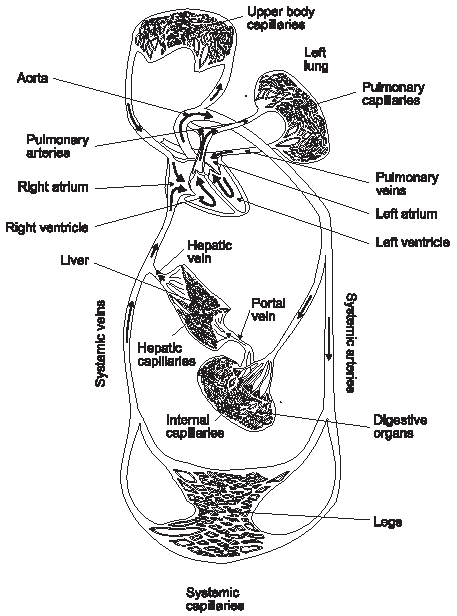
\includegraphics[width=\textwidth]{2_flow_circulatory_system_cropped.pdf}
	\caption[Circulatory system of the human body]{Circulatory system of the human body \cite{JensenUltrasoundBook}}
	\label{fig:2_circulatory_system}
\end{figure}

The flow physics of the human circulatory system are sophisticated and numerous non-stationary flow patterns emerge. The human circulatory system takes care of transporting oxygen and nutrients to the organs as well as disposing of waste products produced by metabolism. It is possible because the blood within the circulatory system contains several smaller subcomponents such as plasma and formed cellular elements that perform these vital functions. Initially, blood is discharged from the left ventricle of the heart via the aorta and travels to all areas of the body via multiple branches of the arterial tree. When the blood flows through the arteries, they into smaller channels known as arterioles. These arterioles lead into a network of tiny capillaries via which nutrients and waste materials are exchanged between the blood and the organs. The capillaries connect to form a network of venulae, which supply the veins, which deliver blood back to the heart. This system, in its totality, is called the systemic circulation. A diagram of the circulatory system as described above, can be seen in \cref{fig:2_circulatory_system}. In summary, when examining the elements that comprise the circulatory system, it consists of several components:
\begin{itemize}
	\item Heart, primary organ of the circulatory system that maintains blood pressure and controls blood velocity.
	\item Blood, and its sub-components
	\begin{itemize}
		\item Plasma, which forms the primary volume and contains nutrients and formed cellular elements.
		\item Red and white blood cells, which carry oxygen and fight off infections, respectively.
		\item Platalets, which are also known as thrombocytes, with the function to clot during a blood vessel injury.
	\end{itemize}
	\item Blood vessels
	\begin{itemize}
		\item Arteries (and arterioles), that transport oxygenised blood to organs and tissues at high pressure and velocity.
		\item Capillaries, thin but wide ranging blood vessels that performs the exchange of matter between the circulatory system and tissue.
		\item Veins (and venules), carries blood back to the heart at low pressure and velocity.
	\end{itemize}
\end{itemize}

\subsection{Blood flow}
Blood flow, which is the amount of blood that goes through a blood vessel in a particular period of time, and has a complicated flow pattern due to its pulsing flow. An advanced analysis of haemodynamics is not within the scope of this report, so the explanation will be brief. The primary forces that determines the blood flow $F$ are the pressure difference across a blood vessel and vascular resistance. It is determined by Ohm's law as in \cref{eq:2_flow_ohms_law}.
\begin{equation} \label{eq:2_flow_ohms_law}
	F = \frac{\Delta P}{R}
\end{equation}
Where $\Delta P$ is the pressure difference across the blood vessel and $R$ is the vascular resistance. The pressure difference $\Delta P$ is calculated with \cref{eq:2_pressure_diff}.
\begin{equation} \label{eq:2_pressure_diff}
	\Delta P = P_{1}-P_{2}
\end{equation}
Where $P_{1}$ and $P_{2}$ are the blood pressures measured at each end of the blood vessel. Pressure has a significant importance on blood flow because an increase in arterial pressure not only increases the force that pushes blood through the capillaries, but it also expands the vessels, lowering vascular resistance.

\section{Devices}
\begin{figure}[ht]
	\centering
	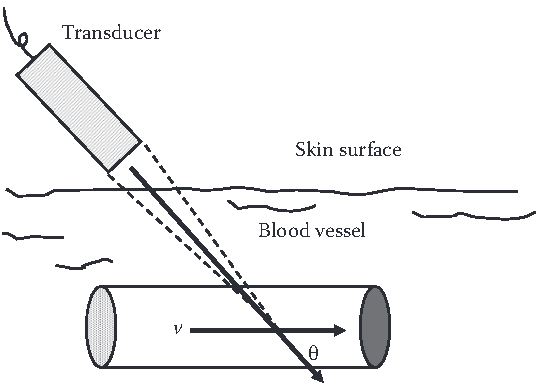
\includegraphics[width=.6\textwidth]{2_ultrasound_scan.pdf}
	\caption[Diagram of ultrasound wave transmitted and reaching blood vessel with incident angle $\theta$]{Diagram of \gls{us} wave transmitted and reaching blood vessel with incident angle $\theta$ \cite{ShungUltrasound_Book}}
	\label{fig:2_ultrasound_flow_scan}
\end{figure}

A device that measures the flowing of blood is called a flowmeter. Flowmeters may be used both inside and outside of vessels. One of the flowmeters that may be used outside the vessel to monitor flow is \gls{us}. \Cref{fig:2_ultrasound_flow_scan} depicts an ultrasonic wave of frequency $f$ insonifying a blood artery, resulting in an angle of $\theta$ relative to velocity $v$. For simplicity, it is assumed that blood flows in a vessel at a constant velocity $v$. The echoes returned are shifted in frequency as described in \cref{eq:2_doppler_theta} in earlier in the chapter.

The echoes scattered by blood after being insonified by an ultrasonic wave convey information about the velocity of blood flow. Blood flow measurements are often used in clinical settings to determine the status of blood vessels and organ functioning. The two commonly used fundamental techniques for ultrasound Doppler flow measurements are \gls{cw} and \gls{pw}. Both will be explained.

\subsection{Continuous-wave flowmeter}
\begin{figure}[ht]
	\centering
	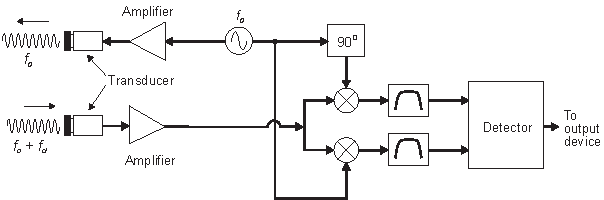
\includegraphics[width=\textwidth]{2_blockdiagram_cwdoppler.pdf}
	\caption[Block diagram of continuous-wave flowmeter]{Block diagram of \gls{cw} flowmeter \cite{JensenUltrasoundBook}}
	\label{fig:2_devices_cw}
\end{figure}
The earliest non-invasive cardiovasclar diagnostic technologies relied heavily on \gls{cw} Doppler flowmeters. One of the earliest concepts for a device to estimate and study blood flow was proposed by \citeauthor{Satomura_CW}\cite{Satomura_CW} during the 1950's in Japan. To continuously transmit waves and receive signals from moving reflectors, the \gls{cw} flowmeter uses two transducers. \gls{cw} flowmeters use less sophisticated electronics than \gls{pw} flowmeters. A drawback to the \gls{cw} flowmeter is the lacking depth discrimination due to the continuous characteristic of this device type. A block diagram of a typical \gls{cw} flowmeter can be seen in \cref{fig:2_devices_cw}.

The basic principles of the device is previously explained in \cref{sec:doppler_effect}, and the measurement of the device is described in \cref{eq:2_doppler_effect}. The device continuously emits an ultrasonic wave in the first transducer expressed as a function of time by \cref{eq:2_cw_tx} \cite{JensenUltrasoundBook}.
\begin{equation} \label{eq:2_cw_tx}
	e(t) = \cos (2\pi f_{0} t)
\end{equation}
While receiving the backscattered signal on the second transducer expressed by \cref{eq:2_cw_rx} \cite{JensenUltrasoundBook}.
\begin{align} \label{eq:2_cw_rx}
	r_{s}(t) &= a \cos \left( 2\pi f_{0} \alpha (t-t_{0}) \right) \\
	\alpha &\approx 1 - \frac{2 v_{z}}{c} \\
	\alpha t_{0} &\approx \frac{2 d_{0}}{c}
\end{align}
Where $v_{z}$ indicates the velocity in the $z$-direction. Applying the Fourier transform, the expression yields \cref{eq:2_cw_fourier}.
\begin{equation} \label{eq:2_cw_fourier}
	r_{s}(t)\cdot e^{j2\pi f_{0} t} \Longleftrightarrow R_{s}(f-f_{0})
\end{equation}
Where $R_{s}(f-f_{0})$ is the Fourier transform of $r_{s}(t)$. The received signal is then multiplied with a quadrature signal of frequency $f_{0}$ to find the Doppler frequency in \cref{eq:2_cw_quadrature}.
\begin{align} \label{eq:2_cw_quadrature}
	m(t) &= a \left[ \cos(2\pi f_{0} t) + j\sin (2\pi f_{0} t) \right] \cos (2\pi f_{0} \alpha (t-t_{0})) \\
	&= \frac{a}{2} \Bigl\{ \cos (2\pi f_{0} [ (1-\alpha) t- \alpha t_{0} ]) + \cos (2\pi f_{0} [ (1-\alpha) t- \alpha t_{0} ]) \\
	&\quad + j \sin (2\pi f_{0} [ (1-\alpha) t- \alpha t_{0} ]) + j \sin (2\pi f_{0} [(1-\alpha) t- \alpha t_{0} ]) \Bigr\} \nonumber
\end{align}

As is general for quadrature demodulation, the resulting signal contains the frequency components of the sum and difference of the emitted and received signals' frequencies shown in \cref{fig:2_demod_fd_frequency_domain}, where the signals are shown in time and frequency domains. 

\begin{figure}[ht]
	\centering
	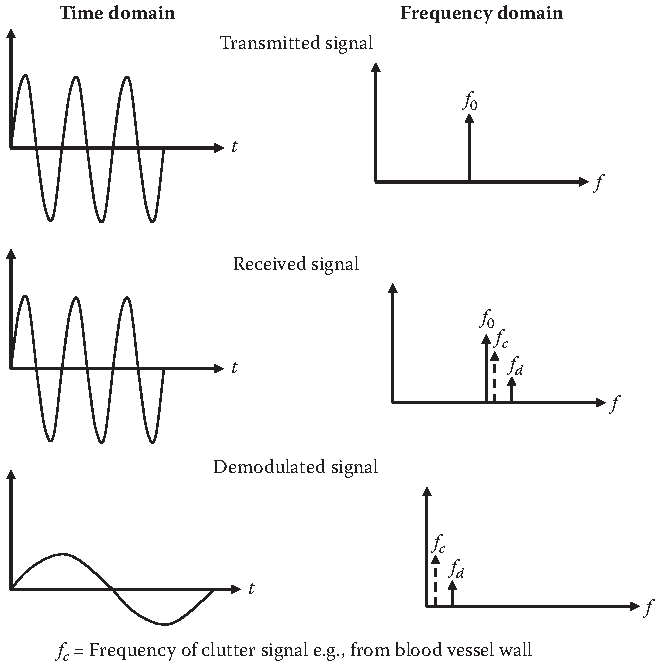
\includegraphics[width=.8\textwidth]{2_demod_fd_frequency_domain-cropped.pdf}
	\caption[Doppler signals in time and frequency domain showing demodulation effects]{Doppler signals in time and frequency domain showing demodulation effects \cite{ShungUltrasound_Book}}
	\label{fig:2_demod_fd_frequency_domain}
\end{figure}

Generally a \gls{bp} filter is used on the demodulated signal to remove the high frequency summed signal at twice the frequency of $f_{0}$. The filtered signal after the \gls{bp} filter is expressed by \cref{eq:2_cw_bp} and contains the Doppler shift of the emitted signal.
\begin{equation} \label{eq:2_cw_bp}
	m_{f}(t) \approx \frac{a}{2} e^{\left(j2\pi f_{0} \frac{2v_{z}}{c}t\right)} e^{\left( -j2\pi f_{0} \alpha t_{0} \right)}
\end{equation}
Where the second exponential term is the delay proportional to the time between transmission and receiving of the signal. The selected cutoff frequency is chosen to be much lower than the carrier frequency to remove the carrier wave. One issue with ultrasonic Doppler blood flow monitoring is that the blood vessels that generate large reflected echoes are also moving with a low velocity. These big, slow-moving echoes are referred to as clutter signals in Doppler nomenclature. The band pass filter's low-end cutoff frequency must be designed to minimize interference from these clutter signals. The design of this band pass filter in the low-frequency region, which serves the function of high pass, also known as a clutter rejection filter, has proven troublesome since the magnitude of clutter signals is many orders greater than that of blood and may obfuscate those from slow-moving blood. 

\begin{table}[ht]
	\centering
	\caption[Measured frequency shifts with a Doppler \qty{3}{\mega\hertz} transducer at various velocities at a \qty{45}{\degree} incident angle]{Measured frequency shifts with a Doppler \qty{3}{\mega\hertz} transducer at various velocities at a \qty{45}{\degree} incident angle \cite{JensenUltrasoundBook}}
	\label{tab:2_cw_frequency_shifts}
	\begin{tblr}[]{%
			width=.3\textwidth,
			colspec = {
				*{1}{S[]}
				*{1}{S[]}
			},
			row{1} = {guard, m, font=\small\bfseries},
			%vlines, hlines,
		}
		\toprule
		{Velocity $\left(v\right)$ \\ \unit[per-mode = symbol]{\meter\per\second}} & {Doppler frequency $\left(f_{d}\right)$ \\ \unit{\hertz} } \\ 
		\midrule
		0.01 & 28 \\
		0.1 & 276 \\
		0.5 & 1377 \\
		1 & 2755 \\
		2 & 5510 \\
		5 & 13770 \\
		\bottomrule
	\end{tblr}
\end{table}

Seen in \cref{tab:2_cw_frequency_shifts} is an example of measured Doppler frequencies using a \qty{3}{\mega\hertz} transducer using the method shown in \cref{fig:2_ultrasound_flow_scan}. Note that the frequencies measured are all within the audible range.

\subsection{Pulsed-wave flowmeter}
\begin{figure}[ht]
	\centering
	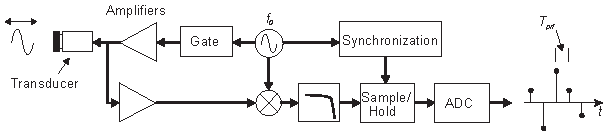
\includegraphics[width=\textwidth]{2_blockdiagram_pwdoppler.pdf}
	\caption[Block diagram of pulsed-wave flowmeter]{Block diagram of \gls{pw} flowmeter \cite{JensenUltrasoundBook}}
	\label{fig:2_devices_pw}
\end{figure}
The concept of a pulsed-wave flowmeter was proposed in \cite{Baker1970} and other related articles. In this type of flowmeter is periodically changing from a transmitter to a receiver. In the transmitting mode, the transducer emits a series of pulses. When in the receiving mode, the transducer is listening for the back-scattered signal. A simplified block diagram can be seen in \cref{fig:2_devices_pw}. The movement of particles within the blood cause a displacement in the back-scattered signal. These systems are commonly referred to as \enquote{Doppler systems} even though it is somewhat misleading. The effects of attenuation is also causing a shift in frequency of a higher magnitude than the velocity of particles in blood. This is because the conventional Doppler effect is not the straight forward methodology that is applied to the analysis of the back-scattered signal. It is, in fact, an artifact. It is the shift in the location of the scatters that is observed, not the shift in the transmitted frequency. \Cref{fig:2_pw_sampling_displacement} shows the received signal after demodulation and filtering; the depth in tissue is fixed here, and the signals displayed on the left side of the figure are the result of a pulse sequence. Each line represents a single pulse, and each pulse is emitted at a pulse repetition frequency, $f_{\textup{prf}}$. Instead, on the right side, the dotted line shows the sampled signal formed by taking into account the amplitude of each pulse after a specified time period.

\begin{figure}[ht]
	\centering
	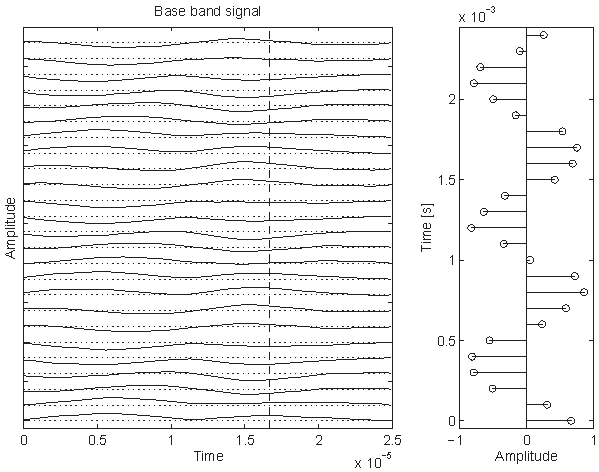
\includegraphics[width=.8\textwidth]{2_pw_pulse_sampling_displacement.pdf}
	\caption[Sampling for a gate pulsed wave system with a single range]{Sampling for a gate pulsed wave system with a single range. To depict the signals on the graph, a single pulse is emitted for each line, and the signals are displaced in amplitude. The sampled signal is displayed on the right. \cite{JensenUltrasoundBook}}
	\label{fig:2_pw_sampling_displacement}
\end{figure}


After the back-scattered signal is received it is multiplied by the center frequency of the emitted pulse and filtered to remove the sum frequency \cite{JensenUltrasoundBook}. A \gls{adc} quantifies the signal for further signal processing. Referring to displacement \cref{fig:2_pw_sampling_displacement} again, the dashed vertical line represents the sample of each pulse that is taken. If sampling is done $T_{s}$ after pulse emission, the measurement depth is expressed by \cref{eq:2_pw_depth}.
\begin{equation} \label{eq:2_pw_depth}
	d_{0} = \frac{T_{s}c}{2}
\end{equation}
Hypothetically, if the velocity of stationary scatterers in blood was measured, a constant amplitude would be measured. A change in sample value is observed when movement is present. Between two pulses the scatterer movement is propertional to the velocity $v_{z}$ in the direction of the ultrasound beam. Time shift of the $t_{s}$ is expressed as \cref{eq:2_pw_timeshift}.
\begin{equation} \label{eq:2_pw_timeshift}
	t_{s} = \frac{2v_{z}}{c}\cdot T_{\textup{prf}}
\end{equation}
Where $c$ is the speed of sound, and $T_{\textup{prf}}$ is the timespan between each pulse emission. Taking one sample from each line at a certain depth yields a sampled signal with a frequency proportional to the scatter velocity. Thus, if a sample is taken at the same depth for each line, resulting in a sinusoidal signal proportional in frequency to the scatter velocity \cite{Munk_Thesis} and that signal is expressed by \cref{eq:2_pw_scatter_velocity_a,eq:2_pw_scatter_velocity_b}.
\begin{subequations}
	\begin{align} 
		r(i) &= a(i) \sin \left( 2\pi f_{p} T_{\textup{prf}} \cdot i \right) \label{eq:2_pw_scatter_velocity_a} \\
		f_{p} &= \frac{2 v_{z}}{c} f_{0} \label{eq:2_pw_scatter_velocity_b}
	\end{align}
\end{subequations}
Where $a(i)$ is the amplitude, $f_{0}$ is the emitted frequency, and $\theta$ is the phase factor in the depth of interest. \todo{Hvor er $\theta$ i udtrykket? Omskriv fra Jensen2012}

This technique improved the accuracy of the investigations of blood vessels and facilitated the display of velocity profiles. Furthermore, employing two transducers or a multi-element transducer, duplex mode imaging (displaying both a B-mode picture and a blood velocity estimate) became feasible. Two-transducer systems are no longer utilised, since it is easier to create a duplex picture with a multi-element transducer. 